\section{Process' perspective}

\subsection{Interactions as developers}
%How do you interact as developers?
Due to the current Covid situation, the team was forced to meet and work online. 
The team typically met on Discord in the DevOps exercise sessions, during the week, and in the weekends. 
Often, collaboration was done through Visual Studio Code's Live Share (which enabled group/pair programming) 
or working through the tasks/exercises individually, helping each other along the way. 
\newline
 
\subsection{Team organization}
%How is the team organized?
The team strived to work in an agile manner, proceeding forward step by step, and adjusting work flows to meet ongoing challenges. 
Mainly, the group worked together as one big group. 
However, occasionally, the group divided into two subgroups to increase efficiency, whereby each subgroup focused on a selected topic. 
Both groups then reconvened to demonstrate and discuss their findings. 
Remaining work was distributed to the individual group members, assisting each other in the process.
  
\subsection{A description of stages and tools included in the CI/CD chains.}%\newline
The tools we used for CI/CD chains were Travis and GitHub Actions. 
We started working with Travis, which worked very well for us. 
Regretably, we experienced some problems with expenses in Travis.
We therefore decided to migrate to GitHub Action which has proven to be just as easy a tool to use as Travis.

\begin{figure}[h!]
    \centering
    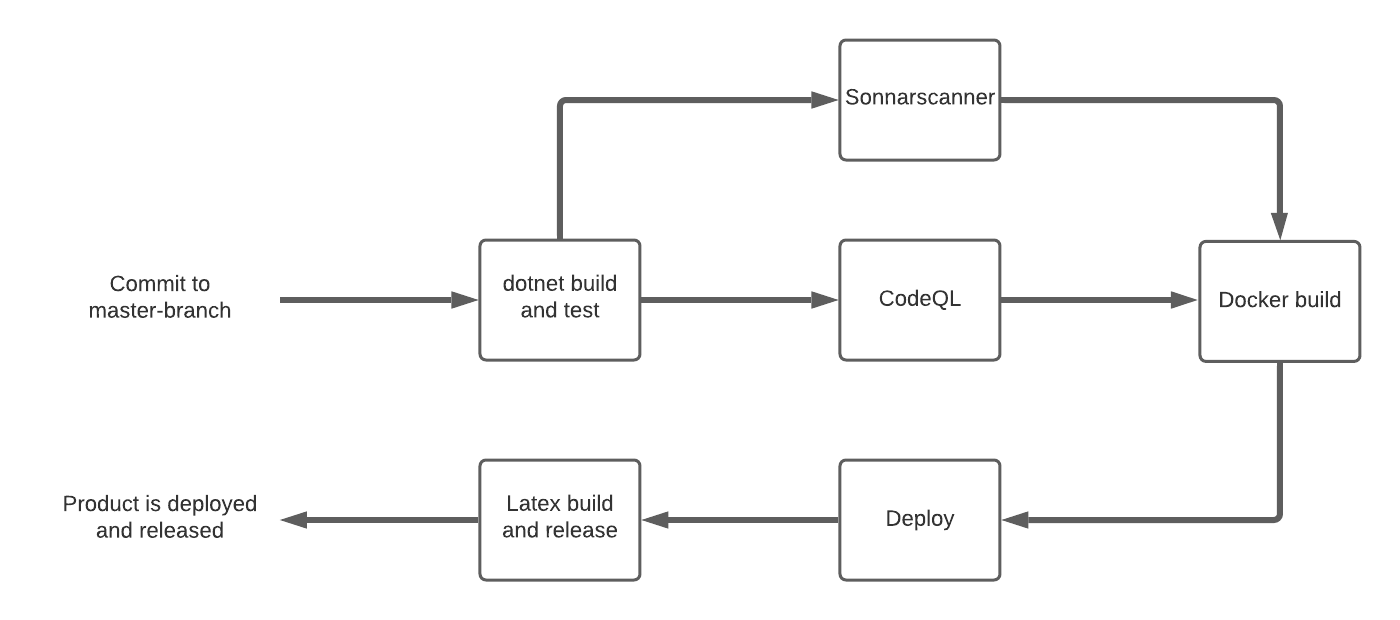
\includegraphics[scale=0.7]{images/CIpipelinediagram.png}
    \caption{An illustration providing an overview of the different steps in our main CI pipeline, used on the masterbranch. }
\end{figure}

Since we are using GitHub anyway to store our repository, GitHub Actions is a good choice since it is easy to 
integrate, easy to duplicate workflow, and has a better ecosystem of actions in Github Marketplace, as well as a centralised app/action store. 
It also provides an accessible way of observing the status of the pipelines, since it is all on GitHub, whereas we had to go to another webpage for Travis.  

The stages in our main workflow are \textit{building and testing}, \textit{CodeQL} that via autobuilds attempts to build any compiled languages, \textit{Sonarscanner} that runs project analysis, \textit{DockerBuild} which build the project, then \textit{deploying} and finally \textit{releasing} it all.\newline

\subsection{Organization of repository} %\newline
For our project we have chosen to use the structure of mono-repository. 
The reason for choosing this structure, was that during this project, we were only building one system. 
Therefore we thought it would be best to keep everything in the same repository, which goes by the name of PythonKindergarten. \newline
  
  
\subsection{Applied branching strategy}
For development purposes, the team uses Git for Distributed Version Control and have adopted a 'long-running branches'-approach to branching. \cite{lecture02}
In this context, there are two main branches, master and develop (i.e. which we have called the 'development' branch) as well as many short-lived topic branches, 
which are used for implementing features. Essentially, the master branch acts as the stable branch and is used for production code and releases whereas the other branches act as the stage for code development. Upon the completion of new features developed on the topic branches, these branches are merged into development and development is later merged into master. This approach to branching works well in a centralized workflow such as ours, where the project is collaborated on in a shared repository (i.e. Github).

The actual process of working with long-running branches in a collaborative setting can present some challenges, especially with regards to eventual merge conflicts whenever branches are merged. 
This can cleary be seen in the instance where, for example, two or more developers have been working on the same code segment(s) on separate branches and alterations have been made. 
Generally, this can be resolved through creating pull requests, and have someone review the code.

\subsection{Applied development process and tools supporting it}
The Projects Board on Github was used to categorize open tasks and organize our development work. Specifically, the team would create an issue with a description added to the comments section, along with labels, such as 'need to have', 'group discussion', etc. attached to it. These same issues were each classified by a tag number and then assigned to different group members. An overview of the current tasks which needed attention (with their current status of either 'To do', 'In Progress' and 'Done') would then be visualized on (either of our two) Projects Boards.

One of the main advantages in working agile is the concept of dividing tasks into sprints. 
Technically, in this project, every week has acted as a mini-sprint as the timespan between each lecture and the assignments that came with it stretched over a week. 
The flexibility of being able to shape and adjust our work flows over such short timespans in order to meet unforeseen contingencies has proven to be quite essential in fulfilling the DevOps 'three ways' of working (as discussed in section 2.1.3 above).  
%\newline

  
\subsection{System monitoring}
Monitoring of our system is done using Prometheus and Grafana, and is deployed using docker-compose. \newline
Prometheus acts as a data collector, periodically scraping metrics from configured targets and storing the collected data in the built-in, local, time series database.\newline
Our system consists of two docker nodes, a master and a worker, which are both configured as targets in our Prometheus deployment.\newline
By configuring our Prometheus server as a datasource within Grafana, the stored time series data can be visualized in preconfigured dashboards. Our metrics are visualized in two separate dashboards, accessible through the Grafana web interface.

To expose metrics in our system we use a NuGet package called prometheus-net \cite{prometheusnet}.
This package allows us to expose metrics on the /metrics endpoint, which can then be scraped and stored by Prometheus.
\newline
To extend the default metrics provided by prometheus-net, we use two additional packages: 
prometheus-net.DotNetMetrics \cite{prometheusdotnetmetrics} and prometheus-net.AspNet \cite{prometheusaspnet}.
\newline
The DotNetMetrics package provides us with general dotnet metrics, such as GC, byte allocation, lock contention and exceptions.
\newline
The AspNet package provides us with ASP.NET specific metrics, such as requests/sec, request duration and error rates.
\newline
\newline
Snapshots of our two dashboards are publicly available on the following links:
\newline
Dotnet metrics: https://tinyurl.com/pythonkindergarten-dotnet
\newline
ASP.NET (api-specific) metrics: https://tinyurl.com/pythonkindergarten-aspnet

\subsection{Logging}
In our system we logged to ElasticSearch from our API, and it used SeriLogs to send these logs. 
We also logged our simulation errors, which we divided into errors regarding follow, tweet, unfollow, connectionError, readTimeout and Register.
In order to aggregate these logs, we used ElasticSearch and Kibana. Additionally, we used ElasticSearch to store our logs in dedicated log indexes, while Kibana was used as a visualization tool for these same logs in ElasticSearch. This made it easy to keep track of our system and we quickly discovered if there was anything wrong. \newline

\subsection{Security assessment}
The identified sources are our web services, used for logging and monitoring, and our MiniTwit application.
Essentially, the servers we used to host were also listed, as well as Docker and Nginx.
The threat sources are XCSS, our firewall (UFW), Docker ignoring UFW and a DDoS attack.
The risk analysis consists of an exposed database connection string, which have been fixed, by storing the connection string as a Docker secret. Our private keys are stored locally on developer machines, but could by mistake be uploaded to GitHub and that would have a catastrophic impact. This would mean one could gain Admin rights to our servers.
Dependency vulnerabilities are also possible, since we do not check versions of our dependencies. Where checking versions in eg. our pipeline, would make it easier to maintain dependencies.
In regards to malicious users gaining access to user data. The impact would be minimized if we kept updates of our database. However we never got to do that.

\subsection{System Scaling and load-balancing}
\subsubsection{Scaling}
We applied both scaling (using docker swarm) and load-balancing (using Digital Ocean's Load Balancer) to our system. 
Our Docker swarm consisted of two servers, a master node and a dedicated worker node, each running multiple service replicas. 
These two servers were internally load-balancing using the Docker routing mesh where only one node needed to be known, in order to communicate with the swarm.

\subsubsection{Load-Balancing}
Situations can occur where every known swarm node is down, in which case the system as a whole might be unreachable, even though there might still be running nodes in the swarm.
\newline
To mitigate this, we used a Digital Ocean Load Balancer. This acted as a gateway (single entry-point) to our Docker swarm, balancing the load between each of our servers and executing health checks, which helped to ensure that the client was always connected to a reachable swarm node.
\newline
We later learned, that we could have gained the same availability benefits, by using heartbeat to coordinate routing of a shared floating ip.
This way we could have ensured that a shared floating ip would always point to an available node in our swarm, while leaving load balancing to the Docker routing mesh. Thus reducing costs and avoiding redundancy.
\newline
As an added bonus, the load balancer masks the ips of our servers from clients, making our system less prone to hackers.

Using these strategies we were able to scale far beyond our current setup, simply by joining more servers to our swarm and configuring these in the DO load balancer.
The only caveat was that our database is currently running on a single server, but could be migrated to a database cluster on Digital Ocean, AWS, Google Cloud or similar cloud providers.

\subsection{From idea to production}

In our group, ideas start of as issues or an observation at group meetings.
To begin with, a developer is assigned and checks out from the development branch, creating a topic branch for the feature.
Whenever a feature is finished being implemented, it is then merged into development.
Sometimes, other features were also merged into development before it was merged into master. 
However, to assure quick release of new features, the branches were most often merged into master immediately. 

The actual deployment process begins when a branch is merged into master, and our CI and CD pipelines can start to run, deploying our product to the production enviroment.
Then the main server, will notify its' worker servers, to update their containers of the running application, with the new docker image. The docker image is pulled from Dockerhub.

Because of how our setup is, we were able to quickly take an idea, develop it, and deploy it to the final product.
This enabled us to quickly push new features to the end user, adhering to the DevOps three way of thinking.
